%
% File eacl2014.tex
%
% Contact g.bouma@rug.nl yannick.parmentier@univ-orleans.fr
%
% Based on the instruction file for ACL 2013 
% which in turns was based on the instruction files for previous 
% ACL and EACL conferences

%% Based on the instruction file for EACL 2006 by Eneko Agirre and Sergi Balari
%% and that of ACL 2008 by Joakim Nivre and Noah Smith

\documentclass[11pt]{article}
\usepackage{eacl2014}
\usepackage{times}
\usepackage{url}
\usepackage{latexsym}
\special{papersize=210mm,297mm} % to avoid having to use "-t a4" with dvips 
%\setlength\titlebox{6.5cm}  % You can expand the title box if you really have to
\usepackage{fancyvrb}
\usepackage{amsmath, amssymb}
\usepackage{graphicx}
\usepackage{array}
\usepackage{multirow}
\usepackage{CJK}
%\usepackage{bera}

\title{A Knowledge-Based Semantic Role Labeling System for Chinese}

\author{First Author \\
  Affiliation / Address line 1 \\
  Affiliation / Address line 2 \\
  Affiliation / Address line 3 \\
  {\tt email@domain} \\\And
  Second Author \\
  Affiliation / Address line 1 \\
  Affiliation / Address line 2 \\
  Affiliation / Address line 3 \\
  {\tt email@domain} \\\And
    Third Author \\
    Affiliation / Address line 1 \\
    Affiliation / Address line 2 \\
    Affiliation / Address line 3 \\
    {\tt email@domain} \\}

\date{}

\begin{document}
\maketitle
\begin{abstract}
We present a knowledge-based semantic role labeling system for Chinese parsed sentences. Our proposed system outperformed the previous reported one from two aspects: knowledge acquisition\{utilization\} and model design. As to the former, the semantic knowledge obtained from E-Hownet were utilized to solve the data sparseness issue; as to the latter, a combination of back-off models was proposed for semantic role classification. They enhanced the performance by 22.45\% and 77.55\%, respectively. Further performance gains through post-processing lead to an overall accuracy improvement from 92.71\% to 94.73\%.           
\end{abstract}
\section{Introduction}
Over the last few years, syntactic parsing paradigms have enjoyed an admirable success, and this has paved the way for semantic parsing. Semantic role labeling (SRL), also known as shallow semantic parsing, is the task of semantically annotating natural language text. Conventionally, a syntactically parsed sentence is taken as input, and semantic arguments associated with predicate of the sentence are identified and classified to a particular semantic class. \cite{Gildea:2002} were the first one to build an automatic SRL system, and since then, their ideas have been dominating the field. In their approach, they emphasized on selection of appropriate lexical and syntactical features for SRL, use of statistical classifiers and their combinations, and ways to handle the data sparseness issue. People have tried to build on that by augmenting and/or altering the feature set \cite{Chen:2003:UDL:1119355.1119361,Xue04calibratingfeatures}, by experimenting with various classification approaches \cite{Park:2005:MEB:1706543.1706583,tan-wang-2009}, and by testing different ways to handle data sparseness concern \cite{Zapirain:2007:USS:1621474.1621551,Lin:2010:CSR:1909632.1912231}. \\
In this study, we follow the traditions to enhance performance of an already reported SRL system for Chinese \cite{you-chen:2004} by (1) enriching its feature set (2) using a semantic knowledge-base to address the data sparseness. However, we take a step further, and propose a different classification approach that is based on a combination of weighted simple probabilistic models. To show the effectiveness of our idea, we build a number of systems that are based on other well established classification approaches (e.g. NaiveBayes, Decision Trees, Maximum Entropy, Linear Interpolation), and compare the outcomes. The experimental results show that our strategy outperformed all other systems, and lead to a considerable improvement in accuracy of the previously reported system.
\section{Experimental Material}
The following two subsections briefly describe the training and testing data we used, and our semantic knowledge source.  
\subsection{Sinica Treebank}
Sinica Treebank \cite{sinica-treebank} is a semantically annotated Chinese tree-bank. In addition to conventional lexical and syntactic annotations, each tree has also been marked for semantic relations of a verbal predicate. It used 74 abstract semantic roles including primary thematic roles (e.g. 'agent', 'theme', etc), secondary roles (e.g. 'location', 'time', 'place', etc), and noun-modification roles (e.g. 'quantifier', 'possessor' etc.). Fig 1 shows an example parse tree from Sinica Treebank.
\begin{figure}[!h]
\centering
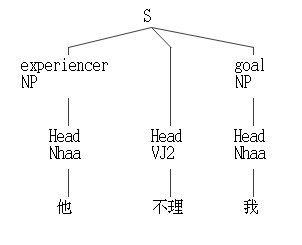
\includegraphics[width=.4\textwidth,height=4cm]{./examples/example5.png}
\caption{An example parsed sentence}
\end{figure}
\subsection{E-HowNet}
E-HowNet\cite{keylist} is a semantic lexical knowledge-base for Chinese. It is an entity-relation model that defines relationships between groups of words ("entities") based on their semantic attributes. It contains n Chinese words which has been grouped into n entities. The grouping, which is based on sense similarity, can be used to generalize lexical statistics. In this study, we have used E-HowNet as our semantic knowledge-source to abate the effects of data sparseness on our SRL system.  
\section{Previous SRL System}
A semantic role labeling (SRL) system for Chinese was reported by \cite{you-chen:2004}. Sinica Treebank was used to train probabilistic models, which, together with a back-off strategy, were used for semantic role classification. As far feature set, the system relied on a number of conventional lexical (i.e. \verb+target word+, \verb+target word pos+, \verb+head word+,  \verb+head word pos+), and syntactic (i.e. \verb+phrase type+,  \verb+position+) features from \cite{Gildea:2002}. %the following conventional lexical and syntactic features:\\[0.2cm]
%\textbf{Lexical Features:}\\
%\verb+h_word:+ Head word\\ 
%\verb+h_pos:+ Part of speech tag of the head word\\ 
%\verb+t_word:+ Target word\\ 
%\verb+t_pos:+ Part of speech tag of the target word\\[0.2cm]
%\textbf{Syntactic Features:} \\ \verb+pt:+ Phrase type\\ 
%\verb+position:+ Position of the target word w.r.t verb  \\[0.2cm]
The overall accuracy of the system was reported to be 92.71\%. Even though this accuracy can be considered on the higher side, there was room for improvement, especially in two subtasks: data sparseness handling and classification approach. We have considerably improved the performance of the system by better addressing the data sparseness issue (Section 4.1), and by proposing a different classification approach (Section 4.3). 
\section{Proposed SRL System}
\subsection{Feature Set}
\textbf{Lexical Features:} \\ 
\verb+t_pos:+ Part of speech tag of the target word\\
\verb+h_pos:+ Part of speech tag of the head word\\ 
\verb+l_r_ch_pos:+ Part of speech tags of the immediate left and right siblings of a test node\\
\verb+all_pos:+ A set of part of speech tags of all nodes under a test node including the test node itself\\[0.2cm]
\textbf{Syntactic Features:} \\ 
\verb+pt:+ phrase type\\
\verb+passive:+ A sentence-level boolean feature indicating weather the sentence, containing the test node, is passive or not\\
\verb+position:+ Position of the target node w.r.t phrasal head\\[0.2cm]
\textbf{Semantic Features:}\\
\verb+h_w_semType:+ Semantic type of the head word extracted from E-HowNet \\ 
\verb+t_w_semType:+ Semantic type of the target word extracted from E-HowNet\\ 
\verb+all_semType:+ A set of semantic types of all nodes of the tree, the test node is a child of\\[0.2cm]
Table 1 shows the values of these features for each constituent of the parse tree shown in Figure 1.
\begin{table}[!h]
\small
\begin{tabular}{|p{2cm}|p{2cm}|p{2cm}|}
\hline \textbf{Semantic Role} & experiencer & goal \\
\hline \verb+t_w_semType+ & 3rdPerson  & speaker \\
\hline \verb+t_pos+ & NP &  NP \\ 
\hline \verb+h_w_semType+ &  ShowInterest & ShowInterest \\ 
\hline \verb+h_pos+ & VJ2 & VJ2 \\ 
\hline \verb+pt+ & S & S \\ 
\hline \verb+position+ & before & after \\ 
\hline \verb+passive+ & false & false \\ 
\hline \verb+l_r_ch_pos+ & empty-VJ2 & VJ2-empty\\ 
\hline \verb+all_pos+ & NP-Nhaa  & NP-Nhaa\\ 
\hline \verb+all_semType+ & 3rdPerson-ShowInterest-speaker  &  3rdPerson-ShowInterest-speaker\\ 
\hline 
\end{tabular}
\caption{Fature-values of each constituent of Figure 1 parse tree}
\normalsize 
\end{table}
\subsection*{Data Sparseness Issue}
As pointed by \cite{Gildea:2002}, lexical statistics, though very useful for semantic role labeling, often becomes a source of data sparseness. For this reason, we have replaced two lexical features (i.e. \verb+head word+, and \verb+target word+) used by the previous system by more general features (i.e. \verb+semType_h_word+ and \verb+semType_t_word+) respectively using E-HowNet. Table 1 gives coverage and the corresponding accuracy statistics before and after adding these generalizations for each of the ten probabilistic models (see Section 4.2 for details of these models). As can be seen, after generalization, the coverage improved considerably for each feature combination, which ultimately resulted in better performance.
\begin{table}[!h]
\small
\begin{center}
\begin{tabular}{|l|l|l|l|l|}
\hline
\multirow{2}{*}{\bf${P_f}_c$} & \multicolumn{2}{|l}{{\bf without E-HowNet}} & \multicolumn{2}{|l|}{\bf with E-HowNet} \\ \cline{2-5} 
                  &   Coverage       &      Accuracy     &     Coverage       &     Accuracy      \\ \hline
   1              &    7.10\%       &    23.61\%       &   12.68\%         &        28.00\%   \\ 
   2              &    52.06\%      &     59.14\%      &   73.05\%         &        74.98\% \\ 
   3              &    67.43\%      &     69.87\%      &   82.68\%         &        81.15\%   \\ 
   4              &    74.56\%       &     68.92\%     &   93.35\%          &        79.16\%  \\ 
   5              &    97.97\%      &      92.25\%     &   97.97\%         &         92.27\%  \\ 
   6              &    28.60\%       &     40.13\%      &  64.20\%          &        62.95\%   \\ 
   7              &    76.30\%       &     68.07\%      &  94.23\%          &        76.87\%  \\ 
   8              &    82.97\%       &      63.50\%     &  96.85\%          &        67.40\%  \\ 
   9              &    99.78\%       &      79.17\%     &   99.78\%         &        79.41\%   \\ 
   10             &    90.09\%       &      58.18\%     &   99.00\%         &          53.31\% \\ \hline
\end{tabular}  
\caption{Coverage \& Accuracy Statistics}
\end{center}
\end{table}
\normalsize

\subsection{Probabilistic Models}
Ten probabilistic models were build using the Sinical treebank labeled data. The probabilities were estimated using the following formula. 
\begin{Verbatim}[commandchars=\\\{\},codes={\catcode`$=3\catcode`_=8}]
  $P(r|constituent)$  
   $= P(r|f_{c})$
   $= #(r,f_{c})/#f_{c}$
\end{Verbatim} 
Where $f_c$ represents a particular feature combination. A number of combinations were tested, and for the final system we used the set of ten combinations given in Table 3.
\begin{table}[!h]
\small
\begin{tabular}{|c|p{6.5cm}|}
\hline \textbf{\#} & \textbf{Feature Combination} \\ 
\hline 1 & \verb+semType_h_w+, \verb+h_pos+, \verb+semType_t_w+, \verb+t_pos+, \verb+pt+, \verb+position+, \verb+all_pos+, \verb+passive+, \verb+all_semType+, \verb+l_r_ch_pos+ \\ 
\hline 2 & \verb+h_pos+, \verb+t_w_semType+, \verb+t_pos+, \verb+pt+, \verb+position+,\verb+passive+\\ 
\hline 3 & \verb+semType_h_w+, \verb+h_pos+, \verb+t_pos+, \verb+pt+, \verb+position+,\verb+passive+\\  
\hline 4 &  \verb+semType_t_w+, \verb+t_pos+, \verb+pt+, \verb+position+,\verb+passive+\\   
\hline 5 &  \verb+semType_h_w+, \verb+semType_t_w+, \verb+pt+, \verb+position+, \verb+passive+\\ 
\hline 6 &  \verb+semType_t_word+, \verb+t_pos+ ,\verb+pt+, \verb+passive+\\ 
\hline 7 &  \verb+semType_t_word+, \verb+t_pos+, \verb+pt+, \verb+passive+ \\ 
\hline 8 &  \verb+semType_t_word+, \verb+t_pos+, \verb+passive+ \\ 
\hline 9 & \verb+t_pos+, \verb+pt+, \verb+position+, \verb+passive+ \\ 
\hline 10  & \verb+semType_t_w+ \\ 
\hline 
\end{tabular} %\begin{verbatim}
\caption{The set of feature combinations}
\normalsize
\end{table}
\subsection{Classification Method}
\subsubsection*{Notations}
\begin{itemize}
\item Let $F$ be the set of ten feature combinations (given in the previous section), and $f_c$ be an element of $F$
\item $P$ be the set of ten corresponding probabilistic models, and ${P_f}_c$ be an element of $P$ that is based on feature combination $f_c$ 
\item ${D_f}_c$ be the probability distribution computed by ${P_f}_c$ 
\item $M_{((p,r)|f_c)}$ be the most probable $(probability,role)$ pair in  ${D_f}_c$
\item $W$ be a set of optimal weights, $w$ be an element of $W$, and $wp$ be a weighted probability (i.e. rank)
\end{itemize} 
\subsubsection*{Algorithm}
Our classification algorithm is as follows:
\begin{enumerate}
\item For a test candidate, extract values of all features (mentioned in section 2) using the parse tree and E-HowNet.
\item initialize $potential\_roles$  $\leftarrow$ $empty$ 
\item For each $f_c$  $\in$ $F$ do:
\begin{itemize}
 \item Find probability distribution ${D_f}_c$ using the corresponding ${P_f}_c$ model
 \item Select $M_{((p,r)|f_c)}$ from ${D_f}_c$
 \item Rank $M_{((p,r)|f_c)}$ by multiplying $p$ with the corresponding $w$ from $W$
 \item Append $(wp,r)$ to $potential\_roles$
 \end{itemize}
\item Return the top ranked $r$ from $potential\_roles$
 \end{enumerate}
\subsection{An Example}
Take the right most node (i.e. 'goal' node) of the parse tree given in Figure 1 as a target node. Below is a brief description of how our proposed method will classify its semantic role.\\
The extracted set of feature values for this node is already given in Table 1 and the probability distribution estimated by each of the ten probabilistic models is given in Table\footnote{Note that due to sparseness of the training data, their are no probability distributions for the feature combination of model 1, 3 and 6.} 3. Note that due to space limitations, and the fact that we are interested only in the roles with heights probability, we give only top 3 roles from the probability distribution wherever applicable.
\begin{table}[!h]
\small
\begin{tabular}{|l|p{6.3cm}|}
\hline \bf ${P_f}_c$ & \bf  Probability Distribution (${D_f}_c$) \\ 
\hline 1 &  \\ 
\hline 2 & [(1.0,'goal')]\\ 
\hline 3 &  \\ 
\hline 4 & [(0.859, 'goal'), (0.107, 'theme'), (0.034, 'range')] \\ 
\hline 5 & [(0.992, 'goal'), (0.008, 'range')]\\ 
\hline 6 & \\ 
\hline 7 & [(0.450, 'agent'), (0.271, 'theme'), (0.177, 'experiencer'), ...] \\ 
\hline 8 & [(0.382, 'agent'), (0.242, 'theme'), (0.152, 'experiencer'), ...]\\ 
\hline 9 & [(0.422, 'goal'), (0.415, 'range'), (0.150, 'theme'), ...] \\ 
\hline 10 & [(0.309, 'agent'), (0.193, 'theme'), (0.121, 'experiencer'), ...] \\ 
\hline 
\end{tabular}  
\caption{Probability distributions}
\end{table}
\noindent Next, from each distribution, we can select $M_{((p,r)|f_c)}$. The full list is given below:
\begin{verbatim}
[NULL,(1.0,'goal'),NULL,
(0.859, 'goal'),(0.992, 'goal'),
 NULL,(0.450, 'agent'),
(0.382, 'agent'),(0.422, 'goal'),
(0.309, 'agent')]
\end{verbatim}
Note that a \verb+NULL+ is inserted for the models that do not have any probability distribution.\\
Finally, each role in this list is ranked by multiplying its probability to the corresponding weight from $W$. These weights encode the worth of a particular feature combination in determining the semantic role, and we have used genetic algorithms and a held out development data-set to find the optimal set (i.e. $W$). The observed optimal set after 100 generations is given below:
\begin{verbatim}
{(w1:0.9),(w2:1.0),(w3:0.9),
(w4:0.7),(w5:0.8),(w6:0.4),
(w7:0.5),(w8:0.4),(w9:0.5),
(w10:0.4)} 
\end{verbatim}
The final list of ranked roles is:
\begin{verbatim}
[NULL,(1.0,'goal'),NULL,
(0.6013, 'goal'),(0.7936, 'goal'),
 NULL,(0.3968, 'agent'),
(0.1528, 'agent'),(0.0764, 'goal'),
(0.03056, 'agent')]
\end{verbatim}
The top ranked \verb+(probability,role)+ pair in this list is \verb+(1.0,'goal')+, hence the role \verb+'property'+ will be assigned to the test node by our classification method.
%\subsection{Discussion}
%A more constrained probabilistic model is supposed to be more reliable for correctness. This might be true in those cases where the role suggested by the more constrained model is also the more probable one. However, in the cases, where a less constrained model suggests a more probable role (as in the above example), there is a trade off between reliability and probability. One way to handle this particular scenario is suggested by our classification method, and that is to rank the roles by multiplying the probabilities to reliability weights and then select the top-ranked role. This approach worked better than the other classification approaches as can be noted from  the experimental results given in the next section.
%One can note that, in the above example, model 5, which is less constrained compared to model 2, suggested a more probable and correct role. This is where our model differed and outperformed the previously reported model. %However, one can argue that more constrained models are supposed to be more reliable. In our approach, this factor is encoded by weights, and we can see that models with more feature constraints tend to have higher weights, while it is the other way around for the less constrained models.  
\section{Experiments and Evaluation}
To evaluate the performance and to show the usefulness of our approach, we have build the following five semantic role labeling systems:
\begin{itemize}
\item \textbf{DT:} Based on Decision Tree classifier
\item \textbf{NB:} Based on Naive Bays classifier
\item \textbf{ME:} Based on Maximum Entropy classifier
\item \textbf{LI:} Based on simple probabilistic models together with linear interpolation
\item \textbf{WPM:} Based on our classification approach
\end{itemize} 
All of these systems were tested using the same feature set (given in Section 4.1), and the same training and testing data (i.e. Sinica Treebank). Results of a 10-fold cross validation scheme are given in Table 3. 
\begin{table}[!h]
\begin{center}
\begin{tabular}{|l|c|c|}
\hline \bf System & \bf Accuracy &  \bf Precision\\ \hline
 DT & 91.03\% & 91.04\%  \\ 
 NB & 92.58\% & 92.57\% \\ 
 ME & 92.67\% & 92.68\% \\ 
 LI & 94.26\% &  94.27\%\\ 
 WPM & 94.49\% & 94.49\% \\ 
\hline 
\end{tabular}
\caption{Evaluation results} 
\end{center}
\end{table}
From the results, we can see that our system outperformed all other systems, and linear interpolation based system is the most competitive one. \\
To further enhance the performance of our system, we added a post-processing component to fix some of the obvious mistakes made by the probabilistic models. One such case is disambiguation between possessor/property roles. We used a heuristic rule that if the semantic type of a target word is \verb+human+, it is more likely to be a \verb+possessor+ than a \verb+property+. With few other such rules, the scores were improved from 94.49\% to 94.73\%. 

\section{Conclusion}
We have presented an improved SRL system for Chinese. We have shown how by using a semantic knowledge-base to handle data sparseness, and by using a weighting strategy to rank the outcomes of simple probabilistic models, the performance of an existing system was enhanced. Together with gains through simple heuristic rules, the overall accuracy was improved from 92.71\% to 94.73\%.
% If you use BibTeX with a bib file named eacl2014.bib, 
% you should add the following two lines:
\clearpage
\bibliographystyle{acl}
\bibliography{eacl2014}

\end{document}
